\section{Introduction}


\begin{frame}{The multiple linear regression model}
    For $i=1,\dots,n$ observations and $k$ regressors,
    \[
        y_i = \beta_0 + \beta_1 x_{i1} + \cdots + \beta_k x_{ik} + \varepsilon_i
    \]

    In matrix form, with $p = k+1$ parameters,
    \[
        \by = \bX\bbeta + \boldsymbol{\varepsilon}, \qquad \boldsymbol{\varepsilon} \sim N(\mathbf{0}, \sigma^2 \mathbf{I})
    \]
    
    \begin{itemize}
        \item $\by$ is $n\times 1$, $\bX$ is $n\times p$, $\bbeta$ is $p\times 1$
        \item The normality assumption is what makes exact $t$ and $F$ inference possible
    \end{itemize}
\end{frame}


\begin{frame}{OLS estimator and its sampling distribution}
    \begin{align*}
        \hat{\bbeta} &= (\bX'\bX)^{-1}\bX'\by \\
        \hat{\bbeta} &\sim N\!\left(\bbeta,\; \sigma^2(\bX'\bX)^{-1}\right)
    \end{align*}
    \begin{itemize}
        \item Write $C_{jj}$ for the $j$th diagonal element of $(\bX'\bX)^{-1}$, so $\Var(\hat\beta_j) = \sigma^2 C_{jj}$
        \item $\sigma^2$ is unknown, so we must estimate it
    \end{itemize}
\end{frame}


\begin{frame}{Estimating $\sigma^2$}
    \begin{align*}
        \hat\sigma^2 = \MSRes = \frac{\SSRes}{n-p}, \qquad \frac{(n-p)\,\MSRes}{\sigma^2} = \frac{\SSRes}{\sigma^2} \sim \chi^2_{n-p}
    \end{align*}
    \begin{itemize}
        \item $\MSRes$ is independent of $\hat{\bbeta}$
        \item Normal divided by an independent $\sqrt{\chi^2/\text{df}}$ gives a $t$ distribution
    \end{itemize}
\end{frame}


% \begin{frame}{Question}
%     What goes wrong with the exact $t$ and $F$ results if the errors are not normal?
%     % \begin{itemize}
%     %     \item Unbiasedness of $\hat{\bbeta}$ and the Gauss--Markov (BLUE) property do not need normality
%     %     \item The exact $t$ and $F$ distributions do need it
%     %     \item For large $n$ the tests are approximately valid by the central limit theorem; for small $n$ with heavy tails or skewness they are not reliable
%     %     \item Prediction intervals are the most sensitive, since they depend on the distribution of a single $\varepsilon_0$, not an average
%     % \end{itemize}
% \end{frame}


\begin{frame}{Running example: delivery time data (MPV Example 3.1)}
    A route driver restocks vending machines. Model the delivery time $y$ (minutes) using $x_1$ = number of cases stocked and $x_2$ = distance walked (feet), $n=25$.
    \begin{table}
        \centering
        \small
        \begin{tabular}{rrrr}
            \toprule
            Obs & $y$ (min) & $x_1$ (cases) & $x_2$ (ft) \\
            \midrule
            1 & 16.68 & 7 & 560 \\
            2 & 11.50 & 3 & 220 \\
            3 & 12.03 & 3 & 340 \\
            4 & 14.88 & 4 & 80 \\
            5 & 13.75 & 6 & 150 \\
            $\vdots$ & $\vdots$ & $\vdots$ & $\vdots$ \\
            25 & 10.75 & 4 & 150 \\
            \bottomrule
        \end{tabular}
    \end{table}
\end{frame}


\begin{frame}[fragile]{Explain this computer output}
    \begin{align*}
        \hat y = 2.3412 + 1.6159\,x_1 + 0.01438\,x_2
    \end{align*}
    \begin{verbatim}
Coefficients:
               Estimate   Std. Error   t value Pr(>|t|)
(Intercept)    2.341231     1.096730     2.135 0.044170
cases          1.615907     0.170735     9.464 3.25e-09
distance       0.014385     0.003613     3.981 0.000631

Residual standard error:   3.259 on 22 degrees of freedom
Multiple R-squared:  0.9596,  Adjusted R-squared:  0.9559
F-statistic: 261.2 on 2 and 22 DF,     p-value: 4.687e-16
    \end{verbatim}
\end{frame}



\section{Test for Significance of Regression}


\begin{frame}{Question}
    We have fitted a model with regressors $x_1,\dots,x_k$. How do we decide whether \emph{any} of them is related to $y$ \emph{in the population}?
    % \begin{itemize}
    %     \item Compare the fitted model with the intercept-only model $y = \beta_0 + \varepsilon$
    %     \item Ask whether the variability explained by the regressors is large relative to the unexplained variability
    % \end{itemize}
\end{frame}


\begin{frame}{Hypotheses for the overall test}
    \begin{align*}
        H_0 &: \beta_1 = \beta_2 = \cdots = \beta_k = 0 \\
        H_1 &: \beta_j \neq 0 \text{ for at least one } j
    \end{align*}
    \begin{itemize}
        \item Under $H_0$ the model reduces to $y = \beta_0 + \varepsilon$
        \item The intercept $\beta_0$ is \emph{not} part of the hypothesis
    \end{itemize}
\end{frame}


\begin{frame}{Decomposing the total variability}
    \begin{align*}
        \SST &= \sum_{i=1}^n (y_i - \bar y)^2 = \by'\by - n\bar y^2 \\
        \SSR &= \hat{\bbeta}'\bX'\by - n\bar y^2 \\
        \SSRes &= \sum_{i=1}^n (y_i - \hat y_i)^2 = \by'\by - \hat{\bbeta}'\bX'\by
    \end{align*}
    \[
        \SST = \SSR + \SSRes
    \]
\end{frame}


\begin{frame}{Degrees of freedom and mean squares}
    \begin{itemize}
        \item $\SST$ has $n-1$ degrees of freedom
        \item $\SSR$ has $k$ degrees of freedom (one per slope)
        \item $\SSRes$ has $n-p = n-k-1$ degrees of freedom
    \end{itemize}
    \begin{align*}
        \MSR = \frac{\SSR}{k}, \qquad \MSRes = \frac{\SSRes}{n-p}
    \end{align*}
\end{frame}


\begin{frame}{Distributional results}
    Under $H_0$ and normal errors,
    \begin{align*}
        \frac{\SSR}{\sigma^2} \sim \chi^2_k, \qquad \frac{\SSRes}{\sigma^2} \sim \chi^2_{n-p}, \qquad \SSR \perp \SSRes
    \end{align*}
    \begin{itemize}
        \item Under $H_1$, $\SSR/\sigma^2$ has a noncentral $\chi^2_k$ distribution
        \item We state these results without proof
    \end{itemize}
\end{frame}


\begin{frame}{The $F$ statistic}
    \begin{align*}
        F_0 = \frac{\SSR/k}{\SSRes/(n-p)} = \frac{\MSR}{\MSRes} \sim F_{k,\,n-p} \quad \text{under } H_0
    \end{align*}
    Reject $H_0$ at level $\alpha$ if $F_0 > F_{\alpha,\,k,\,n-p}$, or equivalently if the $p$-value $P(F_{k,n-p} > F_0)$ is below $\alpha$.
\end{frame}


\begin{frame}{Why a large $F_0$ is evidence against $H_0$}
    Let $\bbeta^* = (\beta_1,\dots,\beta_k)'$ and let $\bX_c$ be the regressor matrix with columns centered at their means.
    \begin{align*}
        E(\MSRes) &= \sigma^2 \\
        E(\MSR) &= \sigma^2 + \frac{\bbeta^{*\prime}\bX_c'\bX_c\bbeta^*}{k}
    \end{align*}
    \begin{itemize}
        \item Under $H_0$ both mean squares estimate $\sigma^2$, so $F_0$ is near 1
        \item Under $H_1$ the extra term is positive, so $F_0$ tends to be large
        \item The test is one-sided: only large values of $F_0$ reject
    \end{itemize}
\end{frame}


\begin{frame}{The ANOVA table}
    \begin{table}
        \centering
        \small
        \begin{tabular}{lllll}
            \toprule
            Source & Sum of squares & df & Mean square & $F_0$ \\
            \midrule
            Regression & $\SSR$ & $k$ & $\MSR$ & $\MSR/\MSRes$ \\
            Residual & $\SSRes$ & $n-p$ & $\MSRes$ & \\
            Total & $\SST$ & $n-1$ & & \\
            \bottomrule
        \end{tabular}
    \end{table}
\end{frame}


\begin{frame}{ANOVA table: delivery time data}
    \begin{table}
        \centering
        \small
        \begin{tabular}{lrrrrr}
            \toprule
            Source & Sum of squares & df & Mean square & $F_0$ & $p$-value \\
            \midrule
            Regression & 5550.81 & 2 & 2775.41 & 261.24 & $4.7\times 10^{-16}$ \\
            Residual & 233.73 & 22 & 10.62 & & \\
            Total & 5784.54 & 24 & & & \\
            \bottomrule
        \end{tabular}
    \end{table}
\end{frame}


\begin{frame}{Decision for the delivery time data}
    \begin{itemize}
        \item Critical value: $F_{0.05,\,2,\,22} = 3.44$
        \item Observed: $F_0 = 261.24 \gg 3.44$, with $p \approx 4.7\times 10^{-16}$
        \item Reject $H_0$: at least one of cases and distance is linearly related to delivery time
        \item The test does not say \emph{which} regressor(s) matter
    \end{itemize}
\end{frame}



\section{Coefficient of Determination}


\begin{frame}{$R^2$ and adjusted $R^2$}
    \begin{align*}
        R^2 &= \frac{\SSR}{\SST} = 1 - \frac{\SSRes}{\SST} \\
        R^2_{\text{adj}} &= 1 - \frac{\SSRes/(n-p)}{\SST/(n-1)}
    \end{align*}
    \begin{itemize}
        \item Delivery time data: $R^2 = 5550.81/5784.54 = 0.9596$ and $R^2_{\text{adj}} = 0.9559$
        \item $R^2$ never decreases when a regressor is added; $R^2_{\text{adj}}$ can
    \end{itemize}
\end{frame}


\begin{frame}{$F_0$ as a function of $R^2$}
    \begin{align*}
        F_0 = \frac{R^2/k}{(1-R^2)/(n-p)}
    \end{align*}
    \begin{itemize}
        \item Delivery time data: $F_0 = \dfrac{0.9596/2}{0.0404/22} = 261.2$
        \item For fixed $k$ and $n$, $F_0$ is increasing in $R^2$: the overall test asks whether $R^2$ is larger than chance alone would produce
    \end{itemize}
\end{frame}


\begin{frame}{Question}
    Delivery time data: $F_0$ is highly significant and $R^2 = 0.96$. Is the model adequate?
    % \begin{itemize}
    %     \item Not necessarily. A significant $F$ only rejects the intercept-only model
    %     \item The relationship may be curved, the variance may be non-constant, or a few points may be driving the fit (observation 9 has $x_1=30$, $x_2=1460$)
    %     \item Residual analysis is needed before trusting any of the inference in this lecture
    % \end{itemize}
\end{frame}



\section{Tests on Individual Coefficients}


\begin{frame}{Question}
    In the simple regression of $y$ on $x_1$ alone, the \(\hat{beta}_1\) is $2.176$. In the multiple regression on $x_1$ and $x_2$, it is $1.616$ ($\hat{\beta}_2$ is $0.014$). Why do they differ?
    % \begin{itemize}
    %     \item In the MLR, $\beta_1$ is the change in mean $y$ per unit of $x_1$ \emph{holding $x_2$ fixed}
    %     \item Cases and distance are correlated ($r = 0.82$), so the SLR slope also absorbs part of the effect of distance
    %     \item Hence a test of $\beta_1 = 0$ in the MLR is a different question from a test of $\beta_1 = 0$ in the SLR
    % \end{itemize}
\end{frame}


\begin{frame}{Hypotheses for an individual coefficient}
    \begin{align*}
        H_0 &: \beta_j = 0 \\
        H_1 &: \beta_j \neq 0
    \end{align*}
    \begin{itemize}
        \item This is a \emph{marginal} (partial) test: it assesses the contribution of $x_j$ given that all the other regressors are already in the model
        \item Changing the other regressors in the model changes the test
    \end{itemize}
\end{frame}


\begin{frame}{Standard error of $\hat\beta_j$}
    \begin{align*}
        \Var(\hat\beta_j) &= \sigma^2 C_{jj} \\
        \operatorname{se}(\hat\beta_j) &= \sqrt{\hat\sigma^2 C_{jj}} = \sqrt{\MSRes\, C_{jj}}
    \end{align*}
    where $C_{jj}$ is the $j$th diagonal element of $(\bX'\bX)^{-1}$.
\end{frame}


\begin{frame}{The $t$ statistic}
    \begin{align*}
        t_0 = \frac{\hat\beta_j}{\operatorname{se}(\hat\beta_j)} \sim t_{n-p} \quad \text{under } H_0
    \end{align*}
    Reject $H_0$ at level $\alpha$ if $|t_0| > t_{\alpha/2,\,n-p}$, or if the two-sided $p$-value $2\,P(t_{n-p} > |t_0|)$ is below $\alpha$.
\end{frame}


\begin{frame}{Testing a general null value}
    For $H_0: \beta_j = \beta_{j0}$,
    \begin{align*}
        t_0 = \frac{\hat\beta_j - \beta_{j0}}{\operatorname{se}(\hat\beta_j)} \sim t_{n-p}
    \end{align*}
    \begin{itemize}
        \item One-sided alternatives $H_1: \beta_j > \beta_{j0}$ or $\beta_j < \beta_{j0}$ use $t_{\alpha,\,n-p}$ and a one-sided $p$-value
    \end{itemize}
\end{frame}


\begin{frame}{Delivery time data: test for cases ($\beta_1$)}
    From $(\bX'\bX)^{-1}$ we get $C_{11} = 0.002744$, and $\MSRes = 10.6242$.
    \begin{align*}
        \operatorname{se}(\hat\beta_1) &= \sqrt{10.6242 \times 0.002744} = 0.1707 \\
        t_0 &= \frac{1.6159}{0.1707} = 9.46
    \end{align*}
    $t_{0.025,\,22} = 2.074$, so $|t_0| > 2.074$ and we reject $H_0: \beta_1 = 0$.
\end{frame}


\begin{frame}{Delivery time data: all coefficients}
    \begin{table}
        \centering
        \small
        \begin{tabular}{lrrrr}
            \toprule
            Term & Estimate & Std.\ error & $t_0$ & $p$-value \\
            \midrule
            Intercept & 2.3412 & 1.0967 & 2.135 & 0.0442 \\
            Cases ($x_1$) & 1.6159 & 0.1707 & 9.464 & $3.3\times 10^{-9}$ \\
            Distance ($x_2$) & 0.014385 & 0.003613 & 3.981 & 0.00063 \\
            \bottomrule
        \end{tabular}
    \end{table}
    At $\alpha = 0.05$ each term is significant given the other regressors.
\end{frame}


\begin{frame}{Interpreting the slopes}
    \begin{itemize}
        \item Each additional case increases mean delivery time by $1.62$ minutes, holding distance fixed
        \item Each additional 100 ft of distance increases mean delivery time by $1.44$ minutes, holding cases fixed
        \item ``Holding the other regressor fixed'' is the whole content of a partial coefficient
    \end{itemize}
\end{frame}


\begin{frame}{Interpreting the intercept}
    \begin{itemize}
        \item $\hat\beta_0 = 2.34$ is the fitted mean time for a delivery with $0$ cases and $0$ ft of distance
        \item The data have $x_1 \in [2, 30]$ and $x_2 \in [36, 1460]$, so the origin is outside the region of the data
        \item Treat $\hat\beta_0$ as a term that positions the fitted plane, not as a physical quantity
    \end{itemize}
\end{frame}


% \begin{frame}{Question}
%     Can the overall $F$ test be significant while every individual $t$ test is insignificant?
%     % \begin{itemize}
%     %     \item Yes. Each $t$ test is conditional on the other regressors, so if $x_1$ and $x_2$ carry nearly the same information, each looks unnecessary given the other
%     %     \item This is a symptom of collinearity, covered later. Here $r(x_1,x_2) = 0.82$ and both are still significant, but $\operatorname{corr}(\hat\beta_1,\hat\beta_2) = -0.82$
%     %     \item Conversely, testing many coefficients at level $\alpha$ each inflates the chance of at least one false rejection
%     % \end{itemize}
% \end{frame}


% \begin{frame}{Preview: $t_0^2$ is a partial $F$ statistic}
%     \[
%         t_0^2 = \frac{\SSR(\beta_j \mid \text{other terms})}{\MSRes}
%     \]
%     Delivery time data, $j=2$: $\SSRes$ is $402.13$ without $x_2$ and $233.73$ with it, so the extra sum of squares is $168.40$.
%     \[
%         t_0^2 = \frac{168.40}{10.6242} = 15.85 = (3.981)^2
%     \]
%     This is the reduced-versus-full model $F$ test with one restriction, developed in the general linear hypothesis section.
% \end{frame}



\section{Confidence Intervals on Coefficients}


\begin{frame}{The pivotal quantity}
    \begin{align*}
        \frac{\hat\beta_j - \beta_j}{\operatorname{se}(\hat\beta_j)} \sim t_{n-p}
    \end{align*}
    \begin{align*}
        P\!\left(-t_{\alpha/2,\,n-p} \le \frac{\hat\beta_j - \beta_j}{\operatorname{se}(\hat\beta_j)} \le t_{\alpha/2,\,n-p}\right) = 1-\alpha
    \end{align*}
\end{frame}


\begin{frame}{Confidence interval for $\beta_j$}
    Solving the inequality for $\beta_j$:
    \begin{align*}
        \hat\beta_j \pm t_{\alpha/2,\,n-p}\, \operatorname{se}(\hat\beta_j)
    \end{align*}
    \begin{itemize}
        \item Interpretation: in repeated sampling, $100(1-\alpha)\%$ of intervals built this way cover the true $\beta_j$
        \item It is a statement about the procedure, not a probability statement about one fixed interval
    \end{itemize}
\end{frame}


\begin{frame}{Delivery time data: 95\% intervals}
    Example for cases: $1.6159 \pm 2.074 \times 0.1707 = (1.262,\, 1.970)$
    \begin{table}
        \centering
        \small
        \begin{tabular}{lrr}
            \toprule
            Term & Lower & Upper \\
            \midrule
            Intercept & 0.0668 & 4.6157 \\
            Cases ($x_1$) & 1.2618 & 1.9700 \\
            Distance ($x_2$) & 0.00689 & 0.02188 \\
            \bottomrule
        \end{tabular}
    \end{table}
\end{frame}


% \begin{frame}{Duality with the $t$ test}
%     \begin{itemize}
%         \item $H_0: \beta_j = \beta_{j0}$ is rejected at level $\alpha$ if and only if $\beta_{j0}$ lies outside the $100(1-\alpha)\%$ interval
%         \item None of the three 95\% intervals contains $0$, matching the three $p$-values below $0.05$
%         \item The intercept interval barely excludes $0$, matching $p = 0.044$
%         \item The interval carries more information: it shows the range of plausible values, not only whether $0$ is one of them
%     \end{itemize}
% \end{frame}


% \begin{frame}{Question}
%     Each of the two slope intervals has 95\% coverage. Do the two intervals \emph{together} have 95\% joint coverage?
%     % \begin{itemize}
%     %     \item No. The probability that both cover simultaneously is at most 95\%, and is generally lower
%     %     \item Bonferroni fix: for $m$ intervals use $t_{\alpha/(2m),\,n-p}$ so that joint coverage is at least $100(1-\alpha)\%$
%     %     \item For the two slopes: $t_{0.0125,\,22} = 2.405$, giving cases $(1.205,\,2.027)$ and distance $(0.00569,\,0.02308)$
%     % \end{itemize}
% \end{frame}


% \begin{frame}{Joint confidence region for $(\beta_1, \beta_2)$}
%     \begin{columns}[T]
%         \column{0.36\textwidth}
%         \begin{itemize}
%             \item Solid ellipse: exact joint 95\% region
%             \item Dashed box: two separate 95\% intervals
%             \item Dotted box: Bonferroni intervals
%             \item The ellipse is tilted because $\operatorname{corr}(\hat\beta_1,\hat\beta_2) = -0.82$
%         \end{itemize}
%         \column{0.64\textwidth}
%         \begin{tikzpicture}
%             \begin{axis}[
%                 width=\linewidth, height=0.72\linewidth,
%                 xlabel={$\beta_1$ (cases)}, ylabel={$\beta_2$ (distance)},
%                 xmin=1.1, xmax=2.15, ymin=0.003, ymax=0.026,
%                 scaled y ticks=false,
%                 yticklabel style={/pgf/number format/fixed, /pgf/number format/precision=3},
%                 tick label style={font=\small}, label style={font=\small},
%             ]
%                 \addplot[thick, domain=0:360, samples=100, smooth]
%                     ({1.615907 + 0.448045*cos(x)}, {0.01438483 - 0.00781494*cos(x) + 0.00536926*sin(x)});
%                 \draw[dashed] (axis cs:1.2618,0.006892) rectangle (axis cs:1.9700,0.021878);
%                 \draw[dotted, thick] (axis cs:1.2052,0.005694) rectangle (axis cs:2.0266,0.023076);
%                 \addplot[only marks, mark=*, mark size=1.8pt] coordinates {(1.615907, 0.01438483)};
%             \end{axis}
%         \end{tikzpicture}
%     \end{columns}
% \end{frame}



\section{Confidence Interval on the Mean Response}


\begin{frame}{Question}
    A new route has $x_1 = 8$ cases and $x_2 = 275$ ft. What is the difference between (a) estimating the \emph{average} delivery time over all such routes and (b) predicting the time of \emph{one particular} such delivery?
    % \begin{itemize}
    %     \item (a) targets a fixed unknown quantity, $E(y \mid \bx_0) = \bx_0'\bbeta$; the only uncertainty is the estimation error in $\hat{\bbeta}$
    %     \item (b) targets a random variable $y_0 = \bx_0'\bbeta + \varepsilon_0$; there is the same estimation error plus the noise $\varepsilon_0$ of that one delivery
    %     \item Same point estimate, different uncertainty, so different intervals
    % \end{itemize}
\end{frame}


\begin{frame}{Point estimate at $\bx_0$}
    Let $\bx_0 = (1, x_{01}, \dots, x_{0k})'$. Then
    \begin{align*}
        \hat y_0 = \bx_0'\hat{\bbeta}
    \end{align*}
    estimates both $E(y \mid \bx_0)$ and the new observation $y_0$.
    \begin{align*}
        \bx_0 = (1, 8, 275)' \;\Rightarrow\; \hat y_0 = 2.3412 + 1.6159(8) + 0.014385(275) = 19.22 \text{ min}
    \end{align*}
\end{frame}


\begin{frame}{Variance of $\hat y_0$ and its distribution}
    \[
        \Var(\hat y_0) = \sigma^2\, \bx_0'(\bX'\bX)^{-1}\bx_0
    \]

    \[
        \frac{\hat y_0 - E(y \mid \bx_0)}{\sqrt{\MSRes\, \bx_0'(\bX'\bX)^{-1}\bx_0}} \sim t_{n-p}
    \]
\end{frame}


\begin{frame}{Confidence interval on the mean response}
    \begin{align*}
        \hat y_0 \pm t_{\alpha/2,\,n-p}\sqrt{\MSRes\, \bx_0'(\bX'\bX)^{-1}\bx_0}
    \end{align*}
\end{frame}


\begin{frame}{Delivery time data at $\bx_0 = (1, 8, 275)'$}
    Here $\bx_0'(\bX'\bX)^{-1}\bx_0 = 0.05397$.
    \begin{align*}
        \text{half-width} &= 2.074\sqrt{10.6242 \times 0.05397} = 1.570 \\
        \text{95\% CI} &= 19.22 \pm 1.57 = (17.65,\, 20.79)
    \end{align*}
\end{frame}



\section{Prediction of New Observations}


\begin{frame}{The forecast error for a new observation}
    \begin{align*}
        y_0 = \bx_0'\bbeta + \varepsilon_0, \qquad \varepsilon_0 \sim N(0,\sigma^2), \quad \varepsilon_0 \perp \hat{\bbeta}
    \end{align*}
    \begin{align*}
        y_0 - \hat y_0 &\sim N\!\left(0,\; \sigma^2\left[1 + \bx_0'(\bX'\bX)^{-1}\bx_0\right]\right)
    \end{align*}
    The extra $\sigma^2$ is the variance of the new observation's own noise $\varepsilon_0$.
\end{frame}


\begin{frame}{Prediction interval}
    \begin{align*}
        \hat y_0 \pm t_{\alpha/2,\,n-p}\sqrt{\MSRes\left[1 + \bx_0'(\bX'\bX)^{-1}\bx_0\right]}
    \end{align*}
    \begin{align*}
        \text{Delivery time data: half-width} &= 2.074\sqrt{10.6242 \times 1.05397} = 6.94 \\
        \text{95\% PI} &= 19.22 \pm 6.94 = (12.28,\, 26.16)
    \end{align*}
\end{frame}


\begin{frame}{Confidence interval versus prediction interval}
    \begin{table}
        \centering
        \small
        \begin{tabular}{lllr}
            \toprule
             & Target & Variance term inside $\sqrt{\cdot}$ & Delivery data at $\bx_0$ \\
            \midrule
            CI & $E(y \mid \bx_0)$ & $\bx_0'(\bX'\bX)^{-1}\bx_0$ & $(17.65,\, 20.79)$ \\
            PI & $y_0$ & $1 + \bx_0'(\bX'\bX)^{-1}\bx_0$ & $(12.28,\, 26.16)$ \\
            \bottomrule
        \end{tabular}
    \end{table}
\end{frame}


\begin{frame}{Question}
    As $n \to \infty$, what happens to the width of the CI on the mean response, and to the width of the PI?

    \pause

    \begin{itemize}
        \item $\bx_0'(\bX'\bX)^{-1}\bx_0 \to 0$, so the CI shrinks to a point: we learn the mean exactly
        \item The PI does not shrink to zero: it tends to $\pm z_{\alpha/2}\,\sigma$, because a new observation still carries its own noise $\varepsilon_0$
    \end{itemize}
\end{frame}


\begin{frame}{CI and PI bands}
    \begin{columns}[T]
        \column{0.34\textwidth}
        Slice of the fitted plane at $x_2 = 275$ ft, as a function of $x_1$.
        \begin{itemize}
            \item Inner band: CI on the mean
            \item Outer band: PI for a new observation
            \item Both bands are narrowest near the center of the data and widen away from it
        \end{itemize}
        \column{0.66\textwidth}
        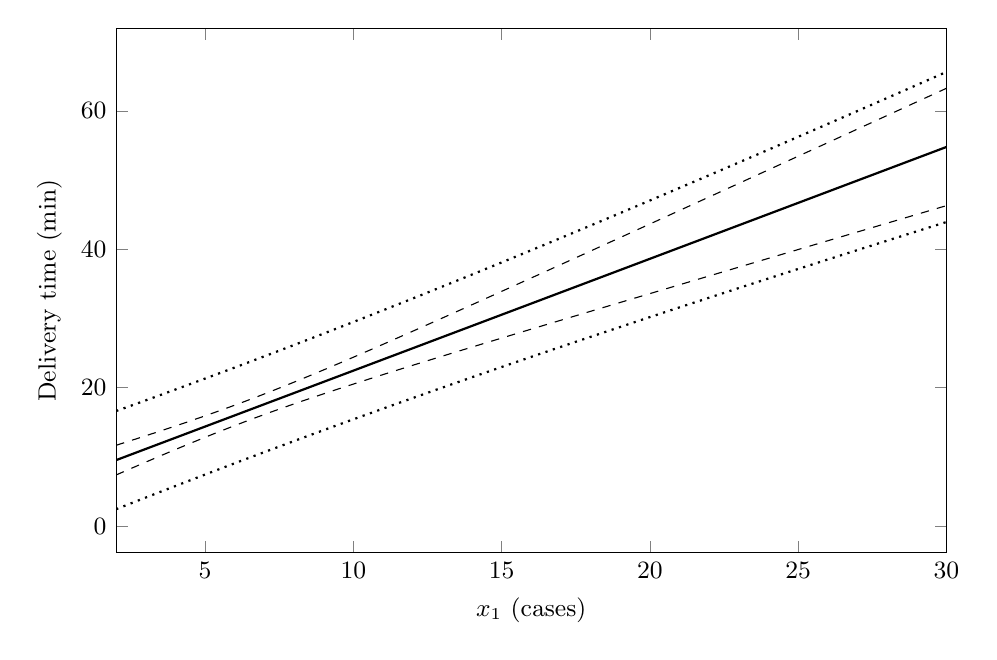
\begin{tikzpicture}
            \begin{axis}[
                width=\linewidth, height=0.68\linewidth,
                xlabel={$x_1$ (cases)}, ylabel={Delivery time (min)},
                xmin=2, xmax=30,
                tick label style={font=\small}, label style={font=\small},
            ]
                \addplot[thick, domain=2:30, samples=60]
                    {6.29706 + 1.615907*x};
                \addplot[dashed, domain=2:30, samples=60]
                    {6.29706 + 1.615907*x + 6.75973*sqrt(0.16011909 - 0.03521858*x + 0.00274378*x^2)};
                \addplot[dashed, domain=2:30, samples=60]
                    {6.29706 + 1.615907*x - 6.75973*sqrt(0.16011909 - 0.03521858*x + 0.00274378*x^2)};
                \addplot[dotted, thick, domain=2:30, samples=60]
                    {6.29706 + 1.615907*x + 6.75973*sqrt(1.16011909 - 0.03521858*x + 0.00274378*x^2)};
                \addplot[dotted, thick, domain=2:30, samples=60]
                    {6.29706 + 1.615907*x - 6.75973*sqrt(1.16011909 - 0.03521858*x + 0.00274378*x^2)};
            \end{axis}
        \end{tikzpicture}
    \end{columns}
\end{frame}


\begin{frame}[fragile]{Prediction in R}
    \begin{verbatim}
new <- data.frame(cases = 8, distance = 275)
predict(fit, new, interval = "confidence")
predict(fit, new, interval = "prediction")

       fit      lwr      upr
  19.22432 17.65390 20.79474
  19.22432 12.28456 26.16407
    \end{verbatim}
    The first output is the CI on the mean response, the second is the PI.
\end{frame}



\section{Hidden Extrapolation}


\begin{frame}{Question}
    Delivery time data: cases range over $[2, 30]$ and distance over $[36, 1460]$. Is a route with $x_1 = 30$ cases and $x_2 = 200$ ft safe to predict for?
    
    \pause

    \begin{itemize}
        \item Each coordinate is inside its own observed range, but the \emph{combination} is not near any observed delivery
        \item The large-case deliveries all have long distances; the model has no information about a 30-case, short-distance route
    \end{itemize}
\end{frame}


\begin{frame}{Regressor variable hull}
    \begin{columns}[T]
        \column{0.4\textwidth}
        Define $h_{00} = \bx_0'(\bX'\bX)^{-1}\bx_0$ and let $h_{\max}$ be the largest diagonal element of the hat matrix $\bX(\bX'\bX)^{-1}\bX'$.
        \begin{itemize}
            \item $h_{00} \le h_{\max}$: $\bx_0$ lies inside the region covered by the data
            \item $h_{00} > h_{\max}$: hidden extrapolation
            \item Dashed polygon: convex hull of the observed $(x_1, x_2)$ pairs
        \end{itemize}
        \column{0.6\textwidth}
        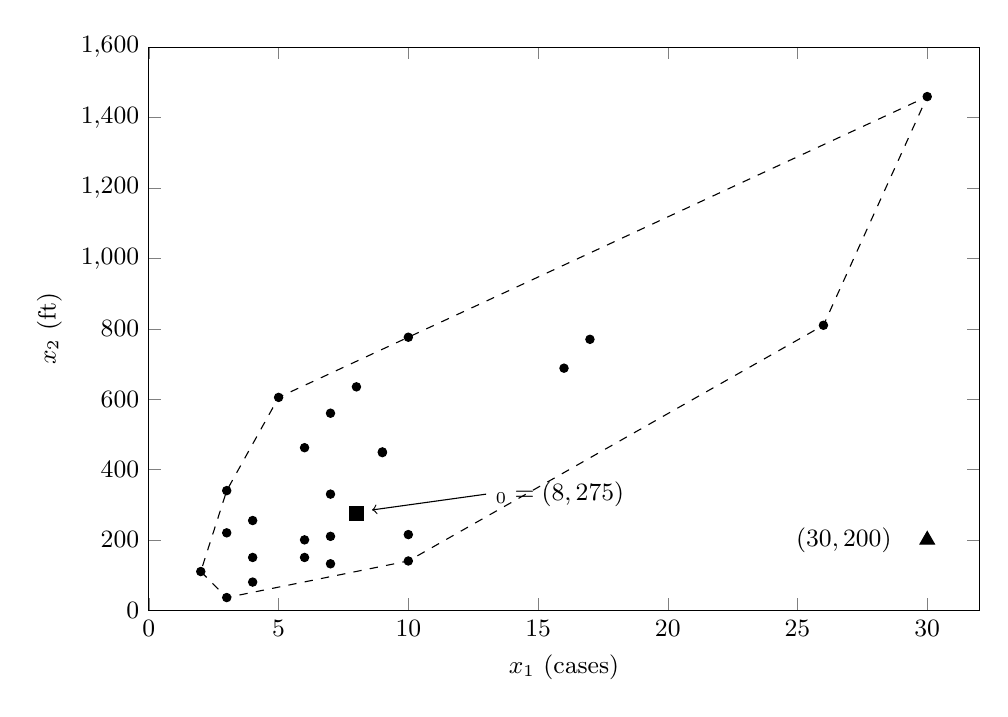
\begin{tikzpicture}
            \begin{axis}[
                width=\linewidth, height=0.72\linewidth,
                xlabel={$x_1$ (cases)}, ylabel={$x_2$ (ft)},
                xmin=0, xmax=32, ymin=0, ymax=1600,
                tick label style={font=\small}, label style={font=\small},
            ]
                \addplot[only marks, mark=*, mark size=1.5pt] coordinates {
                    (7,560) (3,220) (3,340) (4,80) (6,150) (7,330) (2,110) (7,210) (30,1460)
                    (5,605) (16,688) (10,215) (4,255) (6,462) (9,448) (10,776) (6,200) (7,132)
                    (3,36) (17,770) (10,140) (26,810) (9,450) (8,635) (4,150)
                };
                \addplot[dashed] coordinates {(2,110) (3,36) (10,140) (26,810) (30,1460) (5,605) (3,340) (2,110)};
                \addplot[only marks, mark=square*, mark size=2.5pt] coordinates {(8,275)};
                \node[anchor=west, font=\small] (lab) at (axis cs:13,330) {$\bx_0 = (8, 275)$};
                \draw[->, thin] (lab.west) -- (axis cs:8.6,285);
                \addplot[only marks, mark=triangle*, mark size=3pt] coordinates {(30,200)};
                \node[anchor=east, font=\small] at (axis cs:29,200) {$(30, 200)$};
            \end{axis}
        \end{tikzpicture}
    \end{columns}
\end{frame}


\begin{frame}{Checking the two candidate routes}
    Delivery time data: $h_{\max} = 0.498$ (observation 9).
    \begin{table}
        \centering
        \small
        \begin{tabular}{lrrl}
            \toprule
            $(x_{01}, x_{02})$ & $h_{00}$ & $h_{\max}$ & Conclusion \\
            \midrule
            $(8, 275)$ & 0.054 & 0.498 & inside the data region \\
            $(30, 200)$ & 1.757 & 0.498 & hidden extrapolation \\
            \bottomrule
        \end{tabular}
    \end{table}
    For the second route, the CI and PI formulas still compute a number, but the model gives no evidence the fit holds there.
\end{frame}



\section{Summary}


\begin{frame}{Summary of procedures}
    \begin{table}
        \centering
        \small
        \begin{tabular}{llll}
            \toprule
            Procedure & Target & Statistic or interval & Reference \\
            \midrule
            Overall test & $H_0: \beta_1=\cdots=\beta_k=0$ & $F_0 = \MSR/\MSRes$ & $F_{k,\,n-p}$ \\
            $t$ test & $H_0: \beta_j = \beta_{j0}$ & $t_0 = \dfrac{\hat\beta_j - \beta_{j0}}{\operatorname{se}(\hat\beta_j)}$ & $t_{n-p}$ \\[1.5ex]
            CI for $\beta_j$ & $\beta_j$ & $\hat\beta_j \pm t_{\alpha/2,n-p}\operatorname{se}(\hat\beta_j)$ & $t_{n-p}$ \\[0.5ex]
            CI for mean & $E(y \mid \bx_0)$ & $\hat y_0 \pm t_{\alpha/2,n-p}\sqrt{\MSRes\, h_{00}}$ & $t_{n-p}$ \\[0.5ex]
            PI & $y_0$ & $\hat y_0 \pm t_{\alpha/2,n-p}\sqrt{\MSRes(1 + h_{00})}$ & $t_{n-p}$ \\
            \bottomrule
        \end{tabular}
    \end{table}
    with $h_{00} = \bx_0'(\bX'\bX)^{-1}\bx_0$.
\end{frame}
